\documentclass[12pt]{article}
\usepackage{moodle}
\usepackage{fontspec}
\usepackage[brazilian]{babel}
%\usepackage[utf8]{inputenc}
%\usepackage[T1]{fontenc}
\usepackage{graphicx}
\ifwindows\imagemagickcommand{magick convert}
\else\imagemagickcommand{convert}
\fi

\begin{document}
	\begin{quiz}{Mudanças de Fase - Objetiva - Médio}
		\begin{multi}[points=1,penalty=0]{MDF01OM-B}
			\textbf{(FGV/2015)} A água de uma piscina tem 2,0 m de profundidade e superfície com 50 $m^{2}$ de área. Se a intensidade da radiação solar absorvida pela água dessa piscina for igual a 800 $W/m^{2}$, o tempo, em horas, para a temperatura da água subir de 20 ºC para 22 ºC, por efeito dessa radiação, será, aproximadamente, igual a\\
			\textbf{Dados}:\\
			densidade da água = 1 $g/cm^{3}$;\\
			calor específico da água = 1 cal/g.ºC;\\
			1 cal = 4 J.								
			\item 0,8
			\item* 5,6
			\item 1,6
			\item 11
			\item 2,8
		\end{multi}
	
		\begin{multi}[points=1,penalty=0]{MDF02OM-B}
			\textbf{(UDESC/2014)} Analise as proposições sobre o espectro de emissão de radiação do Sol.\\			
			I.	O Sol emite radiação com diferentes frequências, abrangendo um espectro composto por radiações infravermelha, visível e ultravioleta.\\
			II.	A energia da radiação emitida é proporcional a sua frequência, isto é, quanto maior a frequência da radiação maior será a sua energia.\\
			III.	A intensidade da radiação é igual para todas as frequências do espectro de emissão de radiação do Sol, pois, sua magnitude está associada ao inverso do quadrado do raio médio solar.\\
			IV.	A radiação solar que atinge a Terra é caracterizada como monocromática.\\			
			Assinale a alternativa correta.							
			\item Somente as afirmativas III e IV são verdadeiras.
			\item* Somente as afirmativas I e II são verdadeiras.
			\item Somente a afirmativa I é verdadeira.
			\item Somente as afirmativas II e IV são verdadeiras.
			\item Todas as afirmativas são verdadeiras.
		\end{multi}
		\begin{multi}[points=1,penalty=0]{MDF03OM-D}
			\textbf{(UNIFOR CE/2013)} Um condicionado de ar deve manter a temperatura de 20 ºC no interior de um recinto de dimensões 15 m de comprimento, 5 m de largura e 3 m de altura. As paredes do ambiente climatizado têm 25 cm de espessura e condutividade térmica de 0,20 W/m.ºC (ver figura).
			Sabendo que a temperatura exterior é de 40 ºC e que as paredes A, B e C não têm portas e janelas, qual a quantidade de calor, em calorias, a ser extraído por condução do ambiente através das paredes A, B e C pelo condicionado de ar a cada segundo? (considere 1 cal = 4,20 J).
			\begin{center}
				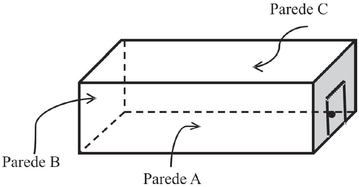
\includegraphics[width=0.7\linewidth]{img2.png}		
			\end{center}							
			\item 385
			\item 390
			\item 395
			\item* 400
			\item 405
		\end{multi}
		\begin{multi}[points=1,penalty=0]{MDF04OM-C}
			\textbf{(Emescam ES/2012)} A crioterapia (terapia do gelo ou utilização do gelo nas lesões) é muito utilizada nas afecções traumáticas, principalmente nas lesões musculoesqueléticas. Ela pode ser chamada de uma modalidade terapêutica, já que é muito utilizada nas reabilitações e na medicina esportiva. Considere uma bolsa plástica que contém gelo em seu ponto de fusão e suponha que a área de contato da bolsa com o corpo de um paciente corresponde a um quadrado de 10 centímetros de lado. A condutividade térmica do plástico é de 0,2 W/m.K e sua espessura é igual a 0,5 mm. Sabendo-se que o paciente está à temperatura constante de 36 °C, podemos afirmar que a quantidade de calor perdida pelo seu corpo para o gelo em 5 minutos de tratamento é de:												
			\item 23200 J
			\item 33200 J
			\item* 43200 J
			\item 53200 J
			\item 63200 J
		\end{multi}
		\begin{multi}[points=1,penalty=0]{MDF05OM-D}
			\textbf{(Unifacs BA/2011)} Como um pregador que anuncia um inferno de “fogo e enxofre”, Nathan S. Lewis vem proferindo um discurso sobre a crise energética que é, ao mesmo tempo, aterrador e estimulante. Para evitar um aquecimento global potencialmente debilitante, o químico do California Institute of Technology, Caltech, afirma que a civilização deve ser capaz de gerar mais de 10 trilhões de joules de energia limpa e livre de carbono até 2050. O Sol lança mais energia sobre a Terra por hora do que a energia que a humanidade consome em um ano. Lewis ressalta que folhas artificiais que captem seus raios e produzam combustível químico em massa no local, de modo muito semelhante ao das plantas, queimem esse combustível para movimentar carros e gerar calor ou energia elétrica.\\
			O laboratório de Lewis é um de vários que produzem protótipos de folhas, não muito maiores que chips de computadores, para produzir combustível de hidrogênio a partir de água, em vez da glicose gerada por folhas naturais. Ao contrário dos combustíveis fósseis, a queima do hidrogênio é limpa. Para abastecer os Estados Unidos de energia, Lewis calcula que, em vez de dispositivos específicos, parecidos com chips, o país precisaria produzir películas de captação solar, finas e flexíveis, que saíssem de linhas de produção de alta velocidade, como jornais. Essas lâminas, ou membranas, deveriam ser de baixo custo como carpetes sob medida e, por fim, cobrir uma área de aproximadamente 53 mil km2, equivalente à superfície da Paraíba, no Brasil.\\ 
			REGALATO, Antonio. A reinvenção da folha vegetal. Disponível em: <http://www.2.uol.com.br/.../a\_reinvenção\_da\_folha\_vegetal.html>. Acesso em: 25 abril 2011.\\			
			Sabendo-se que a intensidade da energia solar que atinge a superfície terrestre é de 0,91 $kW/m^{2}$, é correto afirmar que a energia acumulada, em J, na folha artificial com área de 53 mil $km^{2}$, durante 10,0 h de insolação, incidindo perpendicularmente sobre a superfície, é da ordem de						
			\item $10^{5}$
			\item $10^{8}$
			\item $10^{10}$
			\item* $10^{18}$
			\item $10^{21}$
		\end{multi}	
		\begin{multi}[points=1,penalty=0]{MDF06OM-E}
			\textbf{(UDESC/2010)} Um sistema para aquecer água, usando energia solar, é instalado em uma casa para fornecer 400 L de água quente a 60 °C durante um dia. A água é fornecida para casa a 15 °C e a potência média por unidade de área dos raios solares é 130 $W/m^{2}$. A área da superfície dos painéis solares necessários é:				
			\item 9,50 $m^{2}$
			\item 7,56 $m^{2}$
			\item 2,00 $m^{2}$
			\item 25,0 $m^{2}$
			\item* 6,73 $m^{2}$
		\end{multi}
		\begin{multi}[points=1,penalty=0]{MDF07OM-B}
			\textbf{(UNIOESTE PR/2010)} Num dia de inverno a temperatura no interior de uma casa é 25 ºC e no exterior é 5 ºC. A perda de calor, através de uma janela ($k_{vidro}$ = 0,2 cal/s.m.ºC) de espessura 2 mm e área 0,5 $m^{2}$, em uma hora é						
			\item 3600 cal.
			\item* 3600 kcal.
			\item 36 kcal.
			\item 360 J.
			\item 3600 J.
		\end{multi}
		\begin{multi}[points=1,penalty=0]{MDF08OM-C}
			\textbf{(PUC MG/2007)} Apesar de ser construído de gelo, o iglu é usado pelos esquimós como moradia ou proteção do frio, porque:									
			\item a temperatura do gelo é menor que a do meio ambiente onde vivem os esquimós.
			\item o calor específico do gelo é menor que o da água.
			\item* o gelo não é um bom condutor de calor.
			\item a capacidade térmica do gelo é muito grande.
		\end{multi}
		\begin{multi}[points=1,penalty=0]{MDF09OM-A}
			\textbf{(UEPB/2005)} O matemático e físico francês Jean Baptiste Joseph Fourier (1768- 1830) estudou a condução do calor através de sólidos e publicou, em 1822, a teoria analítica do calor, criando uma lei que levou o seu nome - Lei de Fourier. Observe a seguir, uma aplicação desta teoria.\\
			Um fogão de cozinha elétrico possui entre as paredes do seu forno um isolante constituído por uma camada de fibra de vidro com área total de 1,40 $m^{2}$ e espessura de 4,0 cm . Ao ligar o forno deste fogão, após um certo tempo, a superfície interna da fibra de vidro alcança uma temperatura de 175 ºC e sua superfície externa encontra-se a uma temperatura de 35 ºC . Considerando-se que a condutividade térmica da fibra de vidro é igual a 0,040 W/m, a taxa de transferência de calor através do isolante, em $W/m^{2}$, vale:
			\begin{center}
				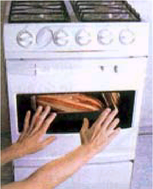
\includegraphics[width=0.3\linewidth]{img5.png}		
			\end{center}											
			\item* 196 
			\item 294 
			\item 130
			\item 150 
			\item 175 
		\end{multi}
		\begin{multi}[points=1,penalty=0]{MDF10OM-A}
			\textbf{(UPE/2009)} Com o objetivo de manter bebidas frias, é utilizada uma caixa de isopor, com área total (incluindo a tampa) de 0,80 $m^{2}$ e espessura da parede de 2 cm. Ela está cheia de gelo e latas de refrigerante, inicialmente a uma temperatura de 0 ºC.\\			
			Dados: k = 0,01 W/m.ºC (condutividade térmica do isopor);\\
			$L_{F}$ = $3,21\times10^{5}$ J/kg (calor de fusão do gelo).\\			
			Se a temperatura da parede externa for mantida a 30 ºC, a quantidade de gelo que se liquefaz durante um dia vale em kg													
			\item* 3,24 
			\item 2,43 
			\item 8,00 
			\item 6,48 
			\item 4,46
		\end{multi}										
	\end{quiz}
\end{document}